% CHAPTER - Analysis ---------------
\chapter{Analysis}%
\label{ch:analysis}
After defining the product specifications, it is possible to start exploring the
solutions space within the project's scope, providing the rationale for viable
solutions and guiding the designer towards a best-compromise solution. In this
chapter are presented the preliminary design and the foreseen tests to
the specifications. 
%
%\section{Product concept}%
%\label{sec:product-concept}
%%\section{Product concept}%
%\label{sec:orge7b0dc6}
The envisioned product consists of a remote controlled vehicle used to assist
exploration and maintenance domains, hereby, denominated as Radio Frequency
Camera Assisted Rover (RFCAR). To satisfy such requirements, the vehicle must
contain a remotely operated camera that provides a live video feed to the user.
Additionally, the vehicle must include an odometric system that assists the
driving and avoids unintentional collisions when remote control is compromised, e.g., when connection is lost.
The vehicle provides means for exploration and conditions assessment in critical
or unaccessible areas to human operators, such as fluid pipelines and other hazardous locations.
%
%%% Local Variables:
%%% mode: latex
%%% TeX-master: "../Phase1"
%%% End:

%%
%\section{Foreseen specifications}%
%\label{sec:fores-spec}
%\section{Foreseen product specifications}%
\label{sec:org31f7574}
In this section the foreseen product specifications of the system to be developed are provided. Such specifications were obtained through the intersection of customer, functional requirements and project restrictions.
\subsection{Quality Function Deployment}%
\label{sec:qfd}
The customer requirements are usually abstract and can collide with the functional requirements, compromising the fulfilment of the project. Thus, it raises the need of a methodology which converts abstract requirements into a series of concrete engineering specifications.

An efficient quality assessment methodology is the use of a Quality House (QFD). In this method, the desired requirements are laid out as rows and the engineering specifications/restrictions as columns. In the intersections lies a symbol representing the strength (weak, moderate or strong --- Figure~\ref{fig:QFD-R} ) of the relationship requirement-specification. This symbol is one of the many tools that allow the quantification of relations existing between the customer requirements and engineering specifications.
For instance, the `engine power' specification and the `fast' requirement have a
very strong correlation (9) since the power of the engine is directly
responsible for the speed of the car.

Along with the requirements, the importance given to each is also specified, ranging from 1 (lowest importance) to 5 (highest importance) these, along with the number at each intersection, will be used to calculate the importance of each specification and thus assign priorities for the Design Team.

Lastly, the triangle shape (the `roof' within the house metaphor) serves as another way of measuring relationships, this time between each specification: such is achieved by placing a symbol (ranging from very negative to very positive, see Figure~\ref{fig:QFD-Roof}) in the diagonal intersection of two specifications. 
I.e., the battery life will have a very negative correlation with the battery temperature, due to the fact that the increase of the temperature will cause a decrease in life time. As such a `very negative' correlation was placed in the diagonal intersection betwixt `Battery Life' and `Battery Temperature'. 
\begin{figure}[!htbp]
   \centering
       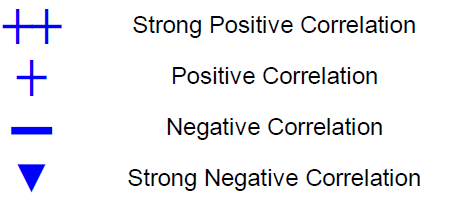
\includegraphics[page=1,width=0.5\textwidth]{sec/img/Roof_Symbols.png} 
 \caption{Quality House - Specification Correlation Strength Symbols}%
\label{fig:QFD-Roof}
\end{figure}

Figure~\ref{fig:QFD} shows the `Quality House' for the RF CAR containing:
\begin{itemize}
\item \textbf{Customer Requirements}: Vehicle Integrity; Obstacle Avoidance; Reliable Feedback; Fast Response; Fast; Budget Friendly; Low Consumption; Small.
\item \textbf{Functional Requirements or Restrictions}: Autonomy; Battery Temperature; Minimum Distance to Obstacle; Maximum Velocity; Motor Expectancy; Cost of Production; Motor Power; Ramp-Up Speed Time; Frame Rate; Camera Range; Resolution; Communication Range; Communication Speed; Dimensions; Mass.
\item \textbf{Intersection Values} (referencing the strength of the requirement-specification correlation) --- see Figure~\ref{fig:QFD-R}.
\item \textbf{Analytical Data}, depicting, in a quantifiable manner, the aims of the project and the relevance of each
  entity:
  \begin{itemize}
  \item Target or Limit Value: The metrics the design team will be based on, white spaces are left for either further discussion and refinement.
  \item Difficulty: Allows a subjective input to be added so that `importance' can be changed to balance unforeseen circumstances.
  \item Importance and Relative Weight: The main conclusion for which the QFD was used, it assigns the priorities for the design team in an objective manner.
  \end{itemize}
\end{itemize}
%
\begin{figure}[!htbp]
   \centering
       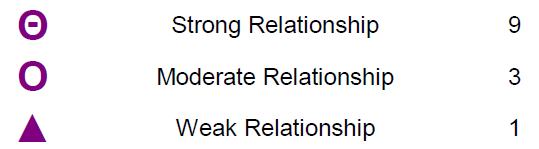
\includegraphics[page=1,width=0.5\textwidth]{sec/img/Relationship_Symbols.png} 
 \caption{Quality House - Relationship Strength Symbols}%
\label{fig:QFD-R}
\end{figure}
%
\begin{sidewaysfigure}[!htbp]
   \centering
       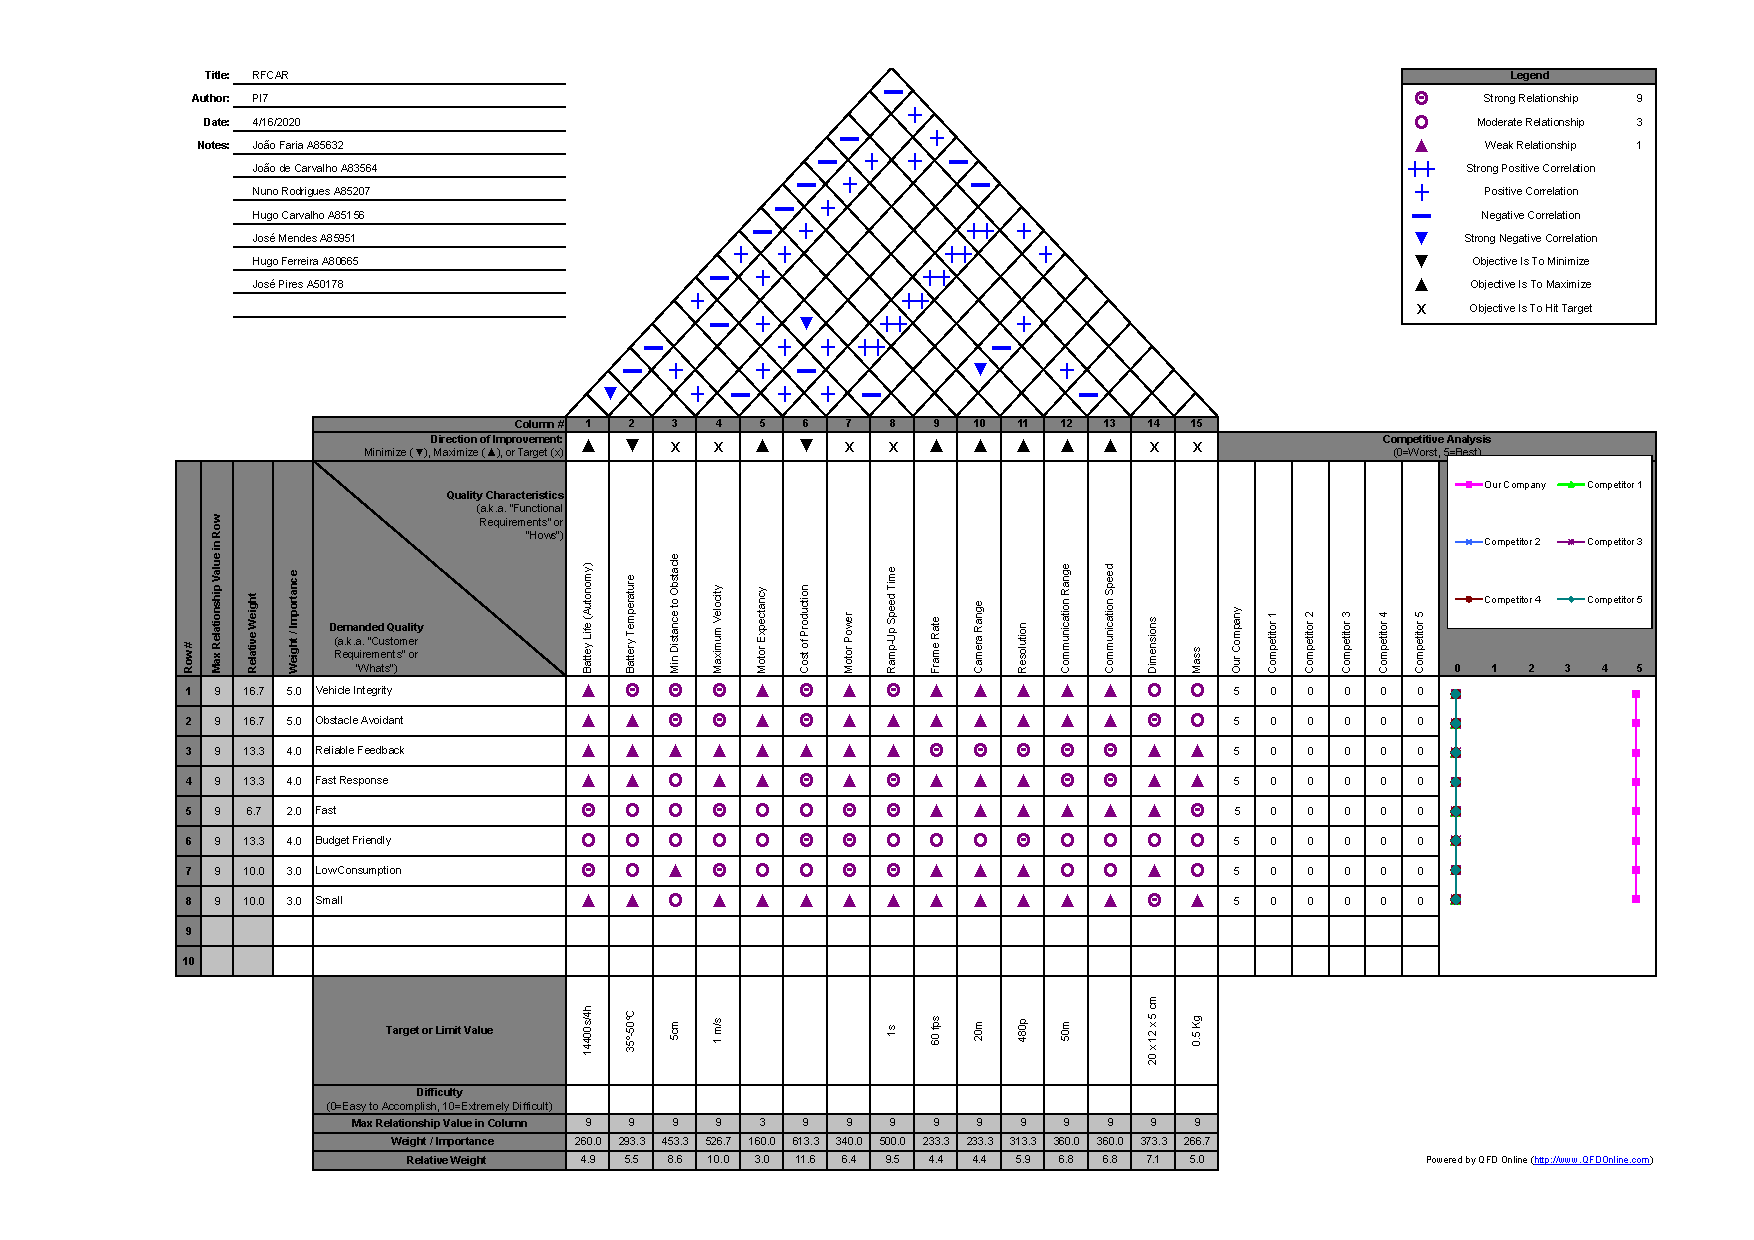
\includegraphics[page=1,width=1.0\textwidth]{sec/pdf/QFDv3.pdf} 
 \caption{Project Study --- RFCar Quality House}%
\label{fig:QFD}
\end{sidewaysfigure}
%
With the QFD, the prioritized ranks and specification targets were obtained and diffused within the Design Team with a
straightforward guideline. For instance, the low cost requirement should be
prioritized over all other specifications, followed by the maximum speed,
Ramp-Up Speed Time and so on.  On the other hand, the engine expectancy is of
little to no consequence (note that the importance added up to a mere 3\%),
followed by the camera-related specifications. This could be regarded as
a point of discussion, which should be prioritized? The functionality of the car
or the the feedback provided by the camera?

With the last point in mind, the QFD has the advantage of promoting further
discussion, simply by changing the importance of a requirement the priority ranking will change, ergo
the priorities can be altered, easily and efficiently, if deemed appropriate.
\newpage
%
\subsection{Vehicle Autonomy}%
\label{sec:autonomy-specs}
The vehicle is operated in wireless mode, thus, a portable power source must be included. The autonomy refers to the vehicle operating hours since the battery is fully charged and safely discharged and should be observed for the following scenarios:
\begin{itemize}
\item No load and vehicle operating at maximum speed;
\item No load and vehicle operating at mean speed;
\item Maximum load and vehicle operating at maximum speed;
\item Maximum load and vehicle operating at mean speed.
\end{itemize}
\subsection{Speed}%
\label{sec:speed-tests}
The vehicle must be operated within a safe range of speed, while also not increasing excessively the power consumption. Thus, these speed boundaries should be tested in the absence of an external load and in the presence of the maximum load.
\subsection{Safety}%
\label{sec:org83942c3}
Vehicle self integrity protection is a requirement in product design, especially considering the vehicle is to
be remotely operated. The safety in the operation can be analysed in two ways, and considers the
preservation of people and goods. For the former, it is important to assure safe interaction as well as user operation --- the vehicle may encounter
several obstacles along its path, but it must not inflict any damage. For the
latter, the vehicle under operating conditions must not inflict any damage to
goods. Thus, in the presence of conflicting user commands violating the safety
of people and goods, the local system should override them, taking corrective
measures to prevent it. The same holds true if the communication between user
and system is lost.
%The system uses odometric navigation.
%\item Human: Due to the odometric sensors safely fixed in the car, crashes will not occur, making it much harder for the car to hit a person or for any part of the car to jump and cause harm to the user or anyone around.
%\end{itemize}
\subsection{Image acquisition}%
\label{sec:image-acquisit}
The vehicle is equipped with a camera to assist in its navigation,
thus, requiring it to be fed to the user's platform appropriately. To do so, several functionalities details need to be addressed efficiently. It was selected the most relevant three and these include the frame rate, the resolution and the image range.
\subsubsection{Frame rate}%
\label{sec:org5adf4ee}
Frame rate refers to the frequency at which independent still images appear on the screen. A better image motion is the result of a higher frame rate but the processing overhead increases as well, so a compromise must be achieved between the quality of the image and the increased processing overhead required. The minimum frame rate defined must be such that allows a clear view of the navigation.
\subsubsection{Range}%
\label{sec:orgecb044c}
How far can the camera capture images without being distorted or unseen by the user. The range must be such that allows the user to see the obstacles when the car is heading to them and provide enough time to change the direction.
\subsubsection{Resolution}%
\label{sec:orgba87554}%
The amount of detail that the camera can capture. It is measured in pixels. The quality of the acquired image is proportional to the number of pixels but a increased resolution requires a greater data transfer and processing overhead, thus, a compromise must be achieved. The minimum resolution must be such that provides the least amount of information required for the user. 
\subsection{Communication}%
\label{sec:org4241610}
For the implementation of the communication, several stages must be considered: Reliability, redundancy and communication range.
\subsubsection{Reliability}%
\label{sec:orgdcb920d}	
A communication is reliable if it guarantees measures to deliver the data
conveyed in the communication link. As reliability imposes these measures, it
also increases memory footprint, which must be considered
depending on the case. For the devised product, an user command
must be acknowledged to be processed, otherwise, the user must be informed; on
the other hand, loosing frames from the video feed is not so critical — user can
still observe conveniently the field of vision if the frame rate is within
acceptable boundaries.
\subsubsection{Redundancy}
\label{sec:orgc5933fc}
The communication protocols are not flawless and the car relies on them to be controlled. If the communication is lost, the car cannot be controlled. A possible solution for this issue is using redundancy in the communication protocols (e.g Wi-Fi and GPRS), so if one protocol fails, the car will still be controlled using the other.
\subsubsection{Range}%
\label{sec:org447a205}
The communication protocols have a limited range of operation, and, as such, regarding the environment on which the car is used the range can be changed.
The range established the maximum distance allowed between user and system for communication purposes.
\subsection{Responsiveness}%
\label{sec:org622e63a}
The movement of the car will be determined by the tilt movement of the smartphone. Sensibility refers to the responsiveness of the car on the minimum smartphone tilt movement. The sensibility must be in an range of values in which small unintentional movements will not be enough to change the state of the car and it does not take big smartphone tilts for the car to move.
\subsection{Closed loop error}%
\label{sec:closed-loop-error-specs}
The speed, direction and safe distance to avoid collisions must be continuously monitored to ensure proper vehicle operation. The closed loop error must then be checked mainly in three situations as a response to an user command:
\begin{itemize}
\item speed: the user issued an command with a given mean speed, which should be compared with the steady-state mean speed of the vehicle.
\item direction: the user issued an command with a given direction, which should be compared to the vehicle direction.
\item safe distance to avoid collisions: the user issued an command with a given direction and speed which can cause it to crash. The local control must influence, to prevent collision, and the final distance to the obstacles must be assessed and compared to the defined one.
\end{itemize}
\subsection{Summary}%
\label{sec:org1f95256}
Table~\ref{tab:specs-init} lists the foreseen product specifications.

% Please add the following required packages to your document preamble:
% \usepackage[table,xcdraw]{xcolor}
% If you use beamer only pass "xcolor=table" option, i.e. \documentclass[xcolor=table]{beamer}
% Please add the following required packages to your document preamble:
% \usepackage[table,xcdraw]{xcolor}
% If you use beamer only pass "xcolor=table" option, i.e. \documentclass[xcolor=table]{beamer}
\begin{table}[!hbt]
\centering
\caption{Specifications}%
\label{tab:specs-init}
%
\begin{tabular}{
>{\columncolor[HTML]{FFFFFF}}l 
>{\columncolor[HTML]{FFFFFF}}l 
>{\columncolor[HTML]{FFFFFF}}l }
\hline
                  & Values     & Explanation                                                                                                  \\ \hline
Autonomy          & 4 h        & \begin{tabular}[c]{@{}l@{}}Time interval between battery fully \\ charged and safely discharged\end{tabular} \\ \hline
Speed Range  & 0.1 to 1 m/s    & \begin{tabular}[c]{@{}l@{}}Speed at which the car can operate\end{tabular}              \\ \hline
Frame Rate        & 60 fps     & \begin{tabular}[c]{@{}l@{}}Frequency at which independent still \\ images appear on the screen\end{tabular}  \\ \hline
Camera Range      & 20 m       & \begin{tabular}[c]{@{}l@{}}How far can the camera capture images\\ without loosing resolution\end{tabular}   \\ \hline
Camera resolution & 480p       & Amount of detail that the camera can capture                                                                 \\ \hline
Communication Range & 50 m & \begin{tabular}[c]{@{}l@{}}Maximum distance between the car and the\\ smarphone without losing connection\end{tabular} \\ \hline
speed Error    & 5 \%       & \begin{tabular}[c]{@{}l@{}}Maximum difference between desired \\ and real speed\end{tabular}              \\ \hline
Direction Error   & 5\%        & \begin{tabular}[c]{@{}l@{}}Maximum difference between desired\\  and real direction\end{tabular}             \\ \hline
Distance Error     & 5 \% & \begin{tabular}[c]{@{}l@{}}Maximum difference between desired\\ and real distance to the obstacle\end{tabular}         \\ \hline
Dimensions        & 20x12x5 cm & Dimensions of the car                                                                                        \\ \hline
Weight            & 0.5 kg     & Weight of the car                                                                                            \\ \hline
\end{tabular}
\end{table}

%%% Local Variables:
%%% mode: latex
%%% TeX-master: "../Phase1"
%%% End:

%
\section{Initial design}%
\label{sec:initial-design}
%\newpage
%\section{Initial design}%
%\label{sec:org68fdd80}
%
Following an analysis family tree of the products(remote controlled cars), the state of the art and the QFD matrix in fig.~\ref{fig:QFD}, an initial design of the product itself can be produced (fig.~\ref{fig:initial-design}).
The selected approach was top-down, in the sense that the requirements and specifications were addressed and that resulted in a general diagram of the product concept. Some macro-level decisions were made in this stage to narrow the solutions pool of the problems, as follows:
\begin{itemize}
\item  The car itself should be battery-powered, as it is a free-moving object that is intended to work in environments where trailing cables could interfere with its regular movement.
\item The device used to control the car should ideally be one already owned by the user, with an integrated screen (e.g.~smartphone), as it would make it more affordable and have a more straightforward interface.
\item The protocols for communication between the controlling device and the Rover should be chosen from within the pool of those readily available to smartphones (e.g. Wi-Fi, GPRS, Bluetooth) to keep the price of the overall product down and make it as practical as possible.
\item  The control and communication unit for the Rover should be divided into two modules: one which can measure and process sensor inputs and control the actuators in real-time, as well as communicate with the user-operated device through a low-latency connection. And another one which can interface directly with the camera module and manage data transmission to the user at the applicational level of the TCP/IP protocol stack, with enough throughput for the specified video resolution and frame rate. The latter should also exchange sensor reading values and commands with the user-controlled device, introducing redundancy to the controls and thus allowing for more reliable operation.
\end{itemize}

\begin{figure}[!ht]
\centering
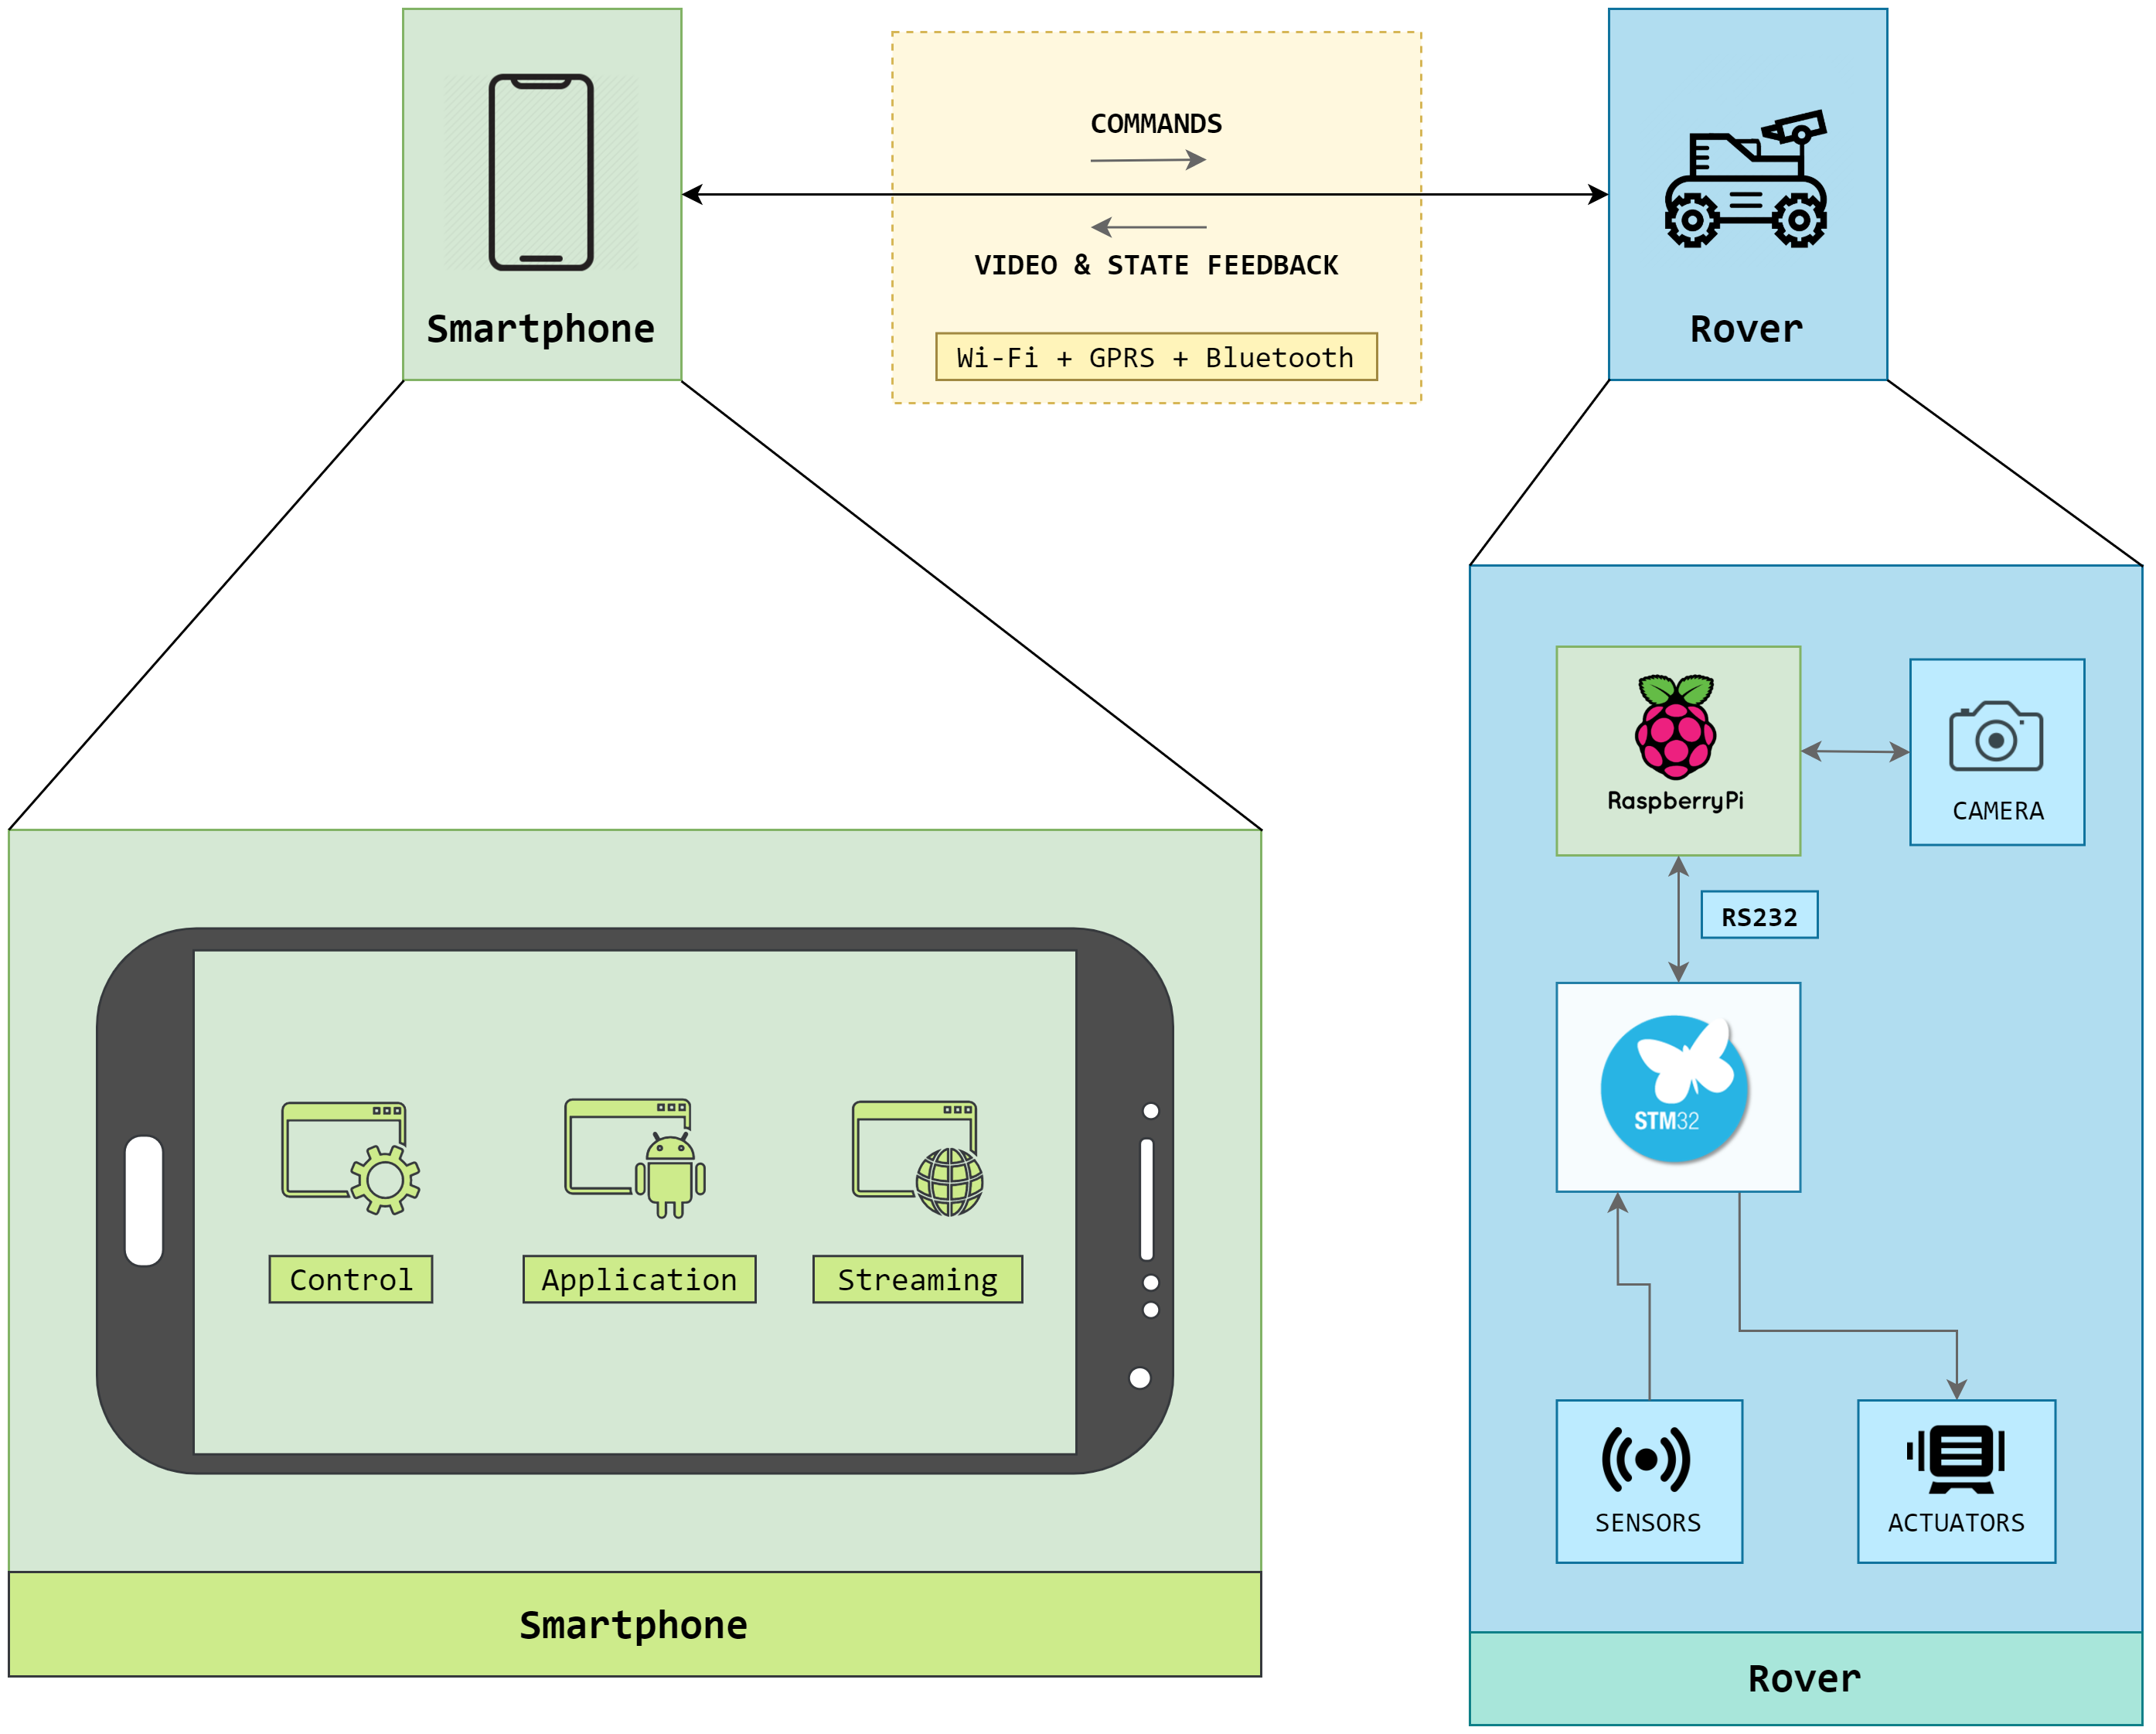
\includegraphics[width=1.0\textwidth]{./sec/img/initial_design_diagram.png}
\caption{\label{fig:initial-design}Initial design: Block diagram view}
\end{figure}

Thus, summarising, the initial design yields the system illustrated in
fig.~\ref{fig:initial-design}, comprised of:

\begin{itemize}
\item \textbf{ Raspberry Pi}: Interfaces with the camera directly, streaming that information to the smartphone. It also receives user commands and sends sensorial information it receives from the STM32 module back to the Smartphone, all through redundant Wi-Fi and GPRS connections;
\item \textbf{STM32}: Receives user commands and sends back sensorial information through a Bluetooth connection, information it also uses to control the actuators;
\item \textbf{Actuators}: DC Motors that control the movement of the Rover and headlights for nocturnal or low light conditions;
\item \textbf{Sensors}: Odometric sensors that support the detection of obstacles and luminosity sensors;
\item \textbf{Camera}: Device connected to the Raspberry Pi that allows the live stream of the car´s surrounding environment;
\item \textbf{Smartphone}: Grant visual feedback from the live feed of the camera also allowing the user to control the movement of the vehicle intuitively;
\end{itemize}

For simulation purposes and in conformance with the extraordinary conditions imposed by the recently enacted confinement measures, the need rose to create a virtual environment to simulate the various subsystems of the Rover. This solution allows for integrated testing without the need to deploy it to the hardware, as illustrated in fig.~\ref{fig:initial-design-2}.

The first of said subsystems is the Physical Environment Virtual Subsystem, which simulates the Rover and the physical environment, also receiving actuator inputs from the Navigation Virtual Subsystem, for which it generates the sensor readings. The latter also exchanges that information, as well as the status of the Rover and the commands from the user with the Smartphone module through a Bluetooth connection, which separates it from the non-simulated environment.

The Remote Vision Virtual Subsystem interfaces with the computer's Web Camera, which is meant to simulate the onboard camera of the Rover. Moreover, it can also communicate through Wi-Fi and GPRS, thus ensuring that communication is kept despite any failure from the Navigation Virtual Subsystem, as well as having shared access to the sensor reading values for monitoring of certain key parameters, depending on their refresh rate.

The RS232 connection between both controlling subsystems ensures proper synchronism and cooperation between them.
\newpage
%\clearpage
\begin{figure}[!ht]
\centering
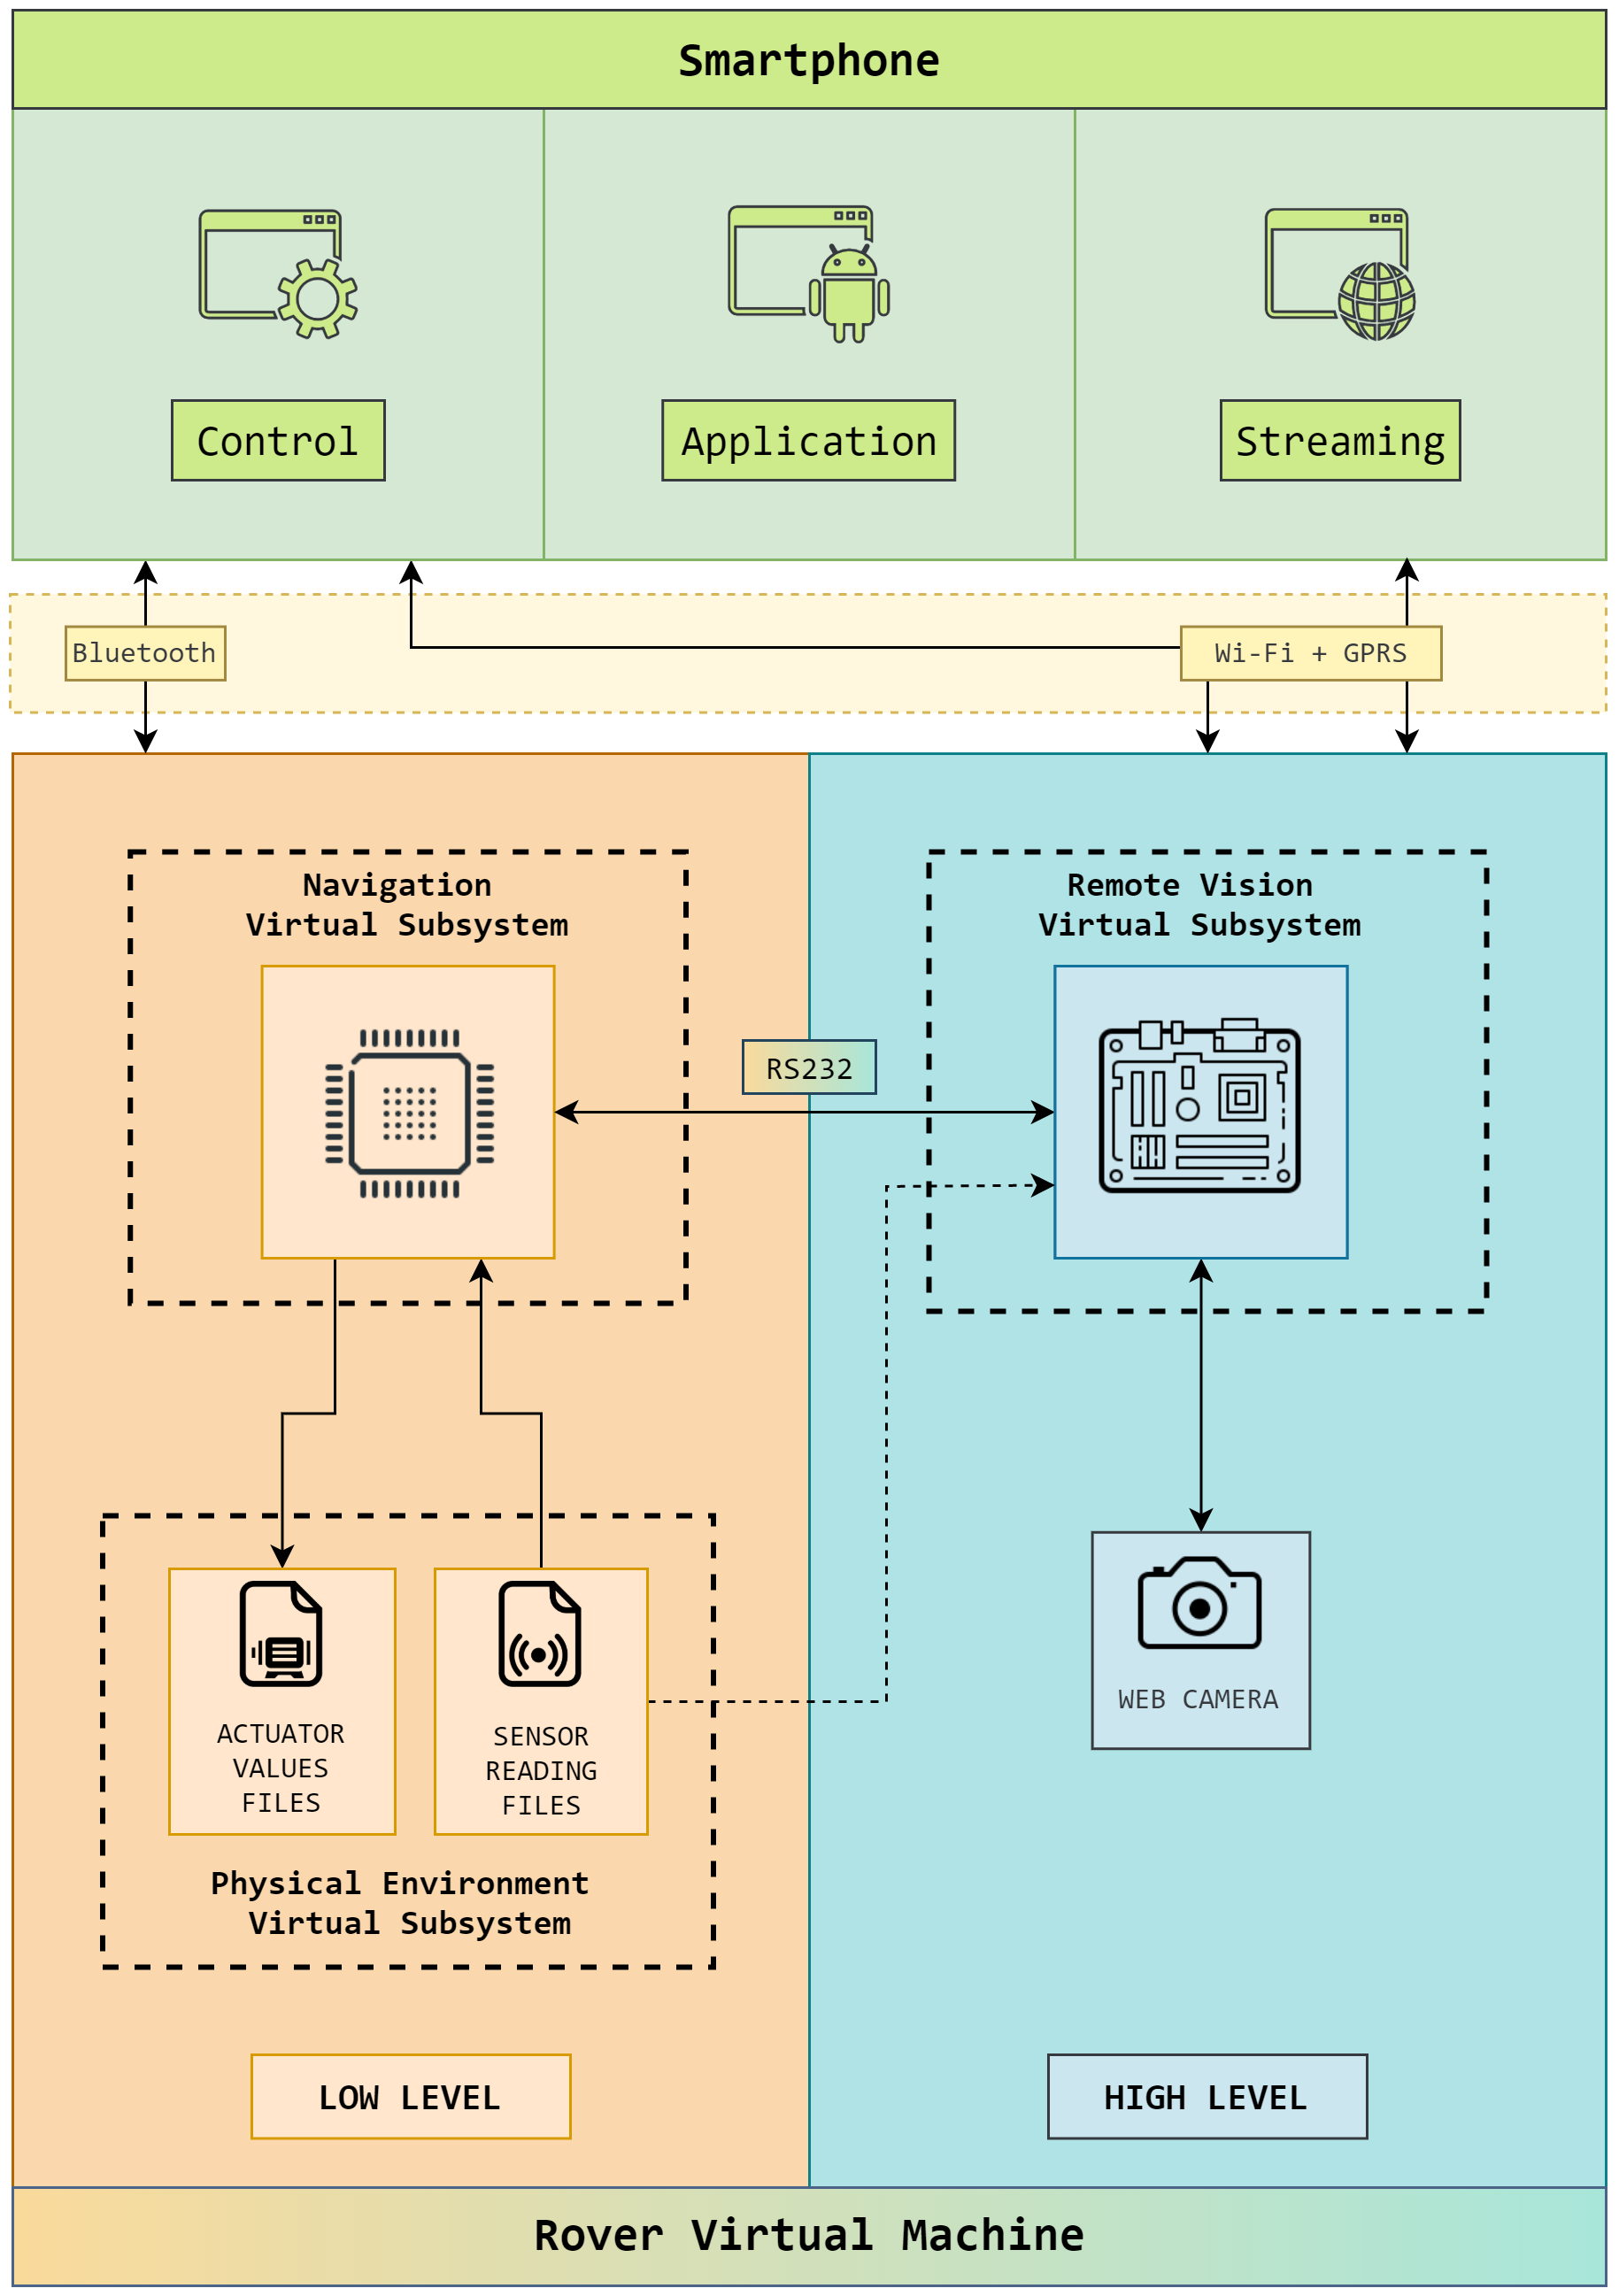
\includegraphics[width=0.85\textwidth]{./sec/img/initial_design_diagram_2.png}
\caption{\label{fig:initial-design-2}Initial design: Virtual environment block diagram view}
\end{figure}

%%% Local Variables:
%%% mode: latex
%%% TeX-master: "../Phase1"
%%% End:
%
\section{Foreseen specifications tests}%
\label{sec:planning}
%\section{Functional testing}%
%\label{sec:org3e2776f}
The functional testing is generally regarded as those performed over any physical
component or prototype. Here, however, a broader sense is used, to reflect the
tests conducted into the system and the several prototypes, under the abnormal
present circumstances.
Moreover, as indicated in the design, the current development
strategy encompasses the virtualization of all hardware components, enclosed
in a single virtual environment.

Thus, it does not make sense to perform
hardware related tests such as velocity measurements, autonomy, safety, etc. As
such, the focus is shifted towards software and control verification,
encompassing the following tests: functionality, image acquisition,
communication, and control algorithms correctness.

The tests are divided into verification and validation tests.
\subsection{Verification tests}%
\label{sec:orge9c79e2}
The verification tests are tests performed internally by the design team to
check the compliance of the foreseen specifications. These tests are done after
the prototype alpha is concluded.

\subsubsection{Functionality}%
\label{sec:functionality}
The remotely operated vehicle is composed of several modules distributed along
several different platforms, some of which distanced from each other.
In doing so, the
proposed sets of functionalities should be tested in the integrated system, by
tracking and analysing the user commands issued along the way until it finally
reaches the vehicle (in the virtual environment), assessing if it is correctly
processed. For example, if the user issues the vehicle to move to a given place
(via smartphone interaction), the message sent to the vehicle must be signalled
in each endpoint hit, and the vehicle should move to that place, symbolically
detected by the modification of its virtual coordinates.

%\subsubsection{Maximum Load}%
%\label{sec:load}
%As mentioned in Section~\ref{sec:load-specs}, the maximum load can be defined
%for the minimum speed (safe motor operation) and for maximum power consuptiom
%increase. Thus, two alternative definitions, and consequently, tests arise for the maximum load determination:
%\begin{enumerate}
%\item maximum load (at minimum speed): maximum load the vehicle can carry
%  safely at the minimum speed defined.
%\item maximum load (at 50\% over the mean power consumption): maximum load which
%  causes a 50\% increase in the mean power consumption, i.e., while operating at
%  mean speed.
%\end{enumerate}
%
%To test the former, load should be increased slowly, measuring the vehicle
%mean speed, until the minimum speed defined is achieved. To test the
%latter, load should be increased slowly, measuring the power consumption, until
%a 50\% increase over the mean power power consumption is detected, while
%operating at the mean speed.
%
%The maximum load can then be defined as the minimum one the vehicle can carry
%while observing both criteria.
%
%\subsubsection{Autonomy}%
%\label{sec:org532616f}
%The autonomy is related to product's power consumption and the capacity of the
%battery chosen. Under the present abnormal circumstances is not reasonable to
%expect the product's power consumption to match the real one, thus, for all
%purposes, this will be considered as the one drawn by the car module itself,
%namely, the installed motors and sensors.
%
%Then, the autonomy can be measured as the time interval between battery fully
%charged and safely discharged (the car stops), by fixating the car to a
%supporting structure with free moving wheels, and imposing the aforementioned
%conditions in Section~\ref{sec:autonomy-specs}.
%
%\subsubsection{Vehicle's Speed}%
%\label{sec:org20789b4}
%The vehicle must be operated within a safe range of speed, as mentioned in
%Section~\ref{speed-tests}.
%The optimum speed maximizes the energy efficiency, increasing battery's life and
%autonomy. The optimum speed must be previously defined through extensive
%vehicle's model simulation. Then, it can be tested experimentally: the vehicle
%must complete a trial track with a sufficiently long
%distance to assure speed reaching and stabilization. The experimental speed is
%then compared to the theorethical speed to measure the error.
%
%and compared to the ones provided in the foreseen specifications.
%The optimum speed maximizes the energy efficiency,
%accounting for the power losses associated with vehicle's dynamics (rolling
%friction, drag, etc.), as well as the increased temperature operation in the
%electronics components
%within a sufficiently long distance to assure speed reach and stabilization,
%and compared to the ones provided in the foreseen specifications.

%\subsubsection{Safety}%
%\label{sec:orgf4c025f}
%As mentioned in Section~\ref{sec:safety-tests}, safety can be analysed in two
%ways, considering the preservation of people and goods.
%
%To test human safety, it is important to identify the interactions between the
%user and the product, and which are the most prevalent and dangerous. Even so,
%the exhaustive test is outside the scope of the present work; a small set of
%features will be tested accordingly to the devised user manual, containing the
%safety measures. For example, battery installation and conditions should be
%tested, eventually leading to the posterior incorporation of safety measures in
%the product.
%
%To test goods safety, it is reasonable to assume the operating conditions of the
%vehicle. Under these it is important to consider the most critical ones that
%concern the moments when the vehicle is left to be controlled locally, instead
%of user controlled operation. The critical conditions for local operations are
%divided into two sets:
%\begin{itemize}
%\item processing of user commands and vehicle operation: user commands can
%  conflict with safety measures and, thus, should be overriden locally.
%\item communication loss: the vehicle is left to odometric navigation,
%  preserving the safety of people and goods.
%\end{itemize}
%To test these two scenarios, they should be replicated, observing the system
%response and tolerance.
%
\subsubsection{Image acquisition}%
\label{sec:orgb1f5c2a}
The vehicle is equipped with remote vision to assist the user in its navigation,
thus, requiring the following variables to be tested: frame rate, range, and
resolution. In the current scenario, the virtual environment should provide
access to a integrated camera, being fairly common nowadays in every modular component, thus, enabling easy testing.

\paragraph{Frame rate}%
\label{sec:frame-rate-test}
To test frame rate, the user screen must be updated with the number of frames
received from the camera per second and checked against the defined boundaries.

\paragraph{Range}%
\label{sec:range-test}
To test camera's range, an object must be captured at increasing distances,
until the object resolution fades or is unclear.

\paragraph{Resolution}%
\label{sec:resolution-test}
The minimum resolution should be tested as providing the least amount of
information required for the user, while minimizing data transfer and processing overhead.

\subsubsection{Communication}%
\label{sec:comm-tests}
The communication tests are performed in compliance to the specifications
provided in Section~\ref{sec:org4241610}, namely reliability and redundancy.

\paragraph{Reliability}%
\label{sec:comm-reliability-test}
To test communication reliability, the most critical communication link is
chosen, namely the wireless communication between user's platform (smartphone)
and vehicle's platform (virtual environment). Then, the communication link and
protocol selected are tested by monitoring the ratio of dropped packets versus
total packets, using an appropriate tool on both directions for transmission and reception.

\paragraph{Redundancy}%
\label{sec:redundancy-test}
To test communication redundancy, one communication channel should be turned
off, verifying if the communication between nodes is still possible through
another communication channel. For example, in the communication between host
(user's platform) and remote (virtual environment) guest systems, the priority
communication is performed between host and high-level subsystem. However, if
this is turned off, the host must also be able to communicate with the remote
system via low-level subsystem.

\subsubsection{Correctness of the control algorithms}%
\label{sec:correct-control-algorithms-test}
As previously mentioned, the speed and position must be continuously monitored
to ensure proper vehicle operation. Under the current circumstances, where the
sensors and actuators are virtualized, the control loops can be externally
stimulated through input files containing the relevant data. Then, the behaviour
of the system can be analysed and verified for some cornercase situations,
assessing the control algorithms correctness.
%
%An overshoot occurs when the output in a control system exceeds its final,
%steady state value generally caused by a sudden change in the system, in this
%case specifically, the placement of a load upon the conveyor will cause an
%overshoot in the latter’s speed which must be controlled lest it cause
%problems.
%
%An overshoot will occur during the settling time, as such, using the same
%considerations taken in its measurement, it can be measured by observing the
%induced voltage at the generator (an overshoot in the conveyor’s speed will
%correspond to a peak in the generator’s voltage).
%
%Using an oscilloscope to display the induced voltage at the generator and making
%use of the “single mode” present in these measuring instruments one can observe
%the change that will occur in the generator’s induced voltage, the peak voltage
%that will be seen when the load is placed upon the running conveyor is the
%electrical representation of the overshoot of speed, then either by
%converting it to its physical representation or comparing it to the reference
%voltage one can arrive at a conclusion. It was agreed that the overshoot
%speed should be \(V_{ss} \pm 10\%\), where \(V_{ss}\) is the stedy state
%speed.

\subsection{Validation tests}%
\label{sec:orgff1a37d}
The validation tests should be performed by the client using the product’s
manual, so it is expected that a user without prior experience with the product
should be able to use it correctly and safely. On the current circumstances,
validation tests should be limited to user interface validation.

For this purpose, an external agent will be provided with the software
application and the respective installation and usage manuals, and the feedback
will be collected and processed to further improve the product.
%%% Local Variables:
%%% mode: latex
%%% TeX-master: "../Phase1"
%%% End:

%
%%% Local Variables:
%%% mode: latex
%%% TeX-master: "../../../dissertation"
%%% End: